\documentclass[12pt]{article}
\usepackage[a4paper, portrait, margin=1cm, right=1cm]{geometry}
\usepackage{fontspec}
\usepackage[fleqn]{amsmath}
\usepackage{setspace}
\usepackage{graphicx}

\graphicspath{./graphics/}
\setmainfont[Ligatures=TeX]{Linux Libertine}

\title{Информационные технологии. Лекция 01. КФС. Основные свойства. БТС}
\author{Студент группы 2305 Макурин Александр}
\date{07 февраля 2023}

\begin{document}

\maketitle
\begin{sloppypar}
    \setstretch{1.8}

    \section*{Организационные вопросы}
    \subsection*{Список лабораторных (каждая даёт 10 баллов)}
    \begin{itemize}
        \item Начало работ с Gazebo
        \item Создание модели ТС (БПЛА, БТС)
        \item Автономное ТС
        \item Реализация протоколов связи
        \item Роевой интеллект на группе ТС
        \item Стратегическое планирование
    \end{itemize}
    \subsection*{Оценки}
    \begin{itemize}
        \item 95\%+ (57+ баллов) = 5
        \item 90\%+ (54+ баллов) = 4
        \item 80\%+ (48+ баллов) = 3
    \end{itemize}

    \section*{Индустрия 4.0 - замещение людей роботами в производстве}

    БТС - беспилотное транспортное средство

    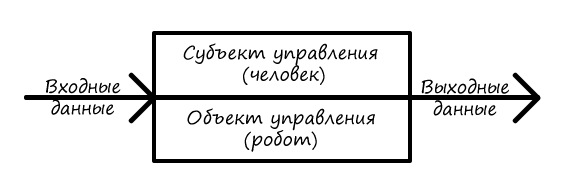
\includegraphics[width=0.5\textwidth]{graphics/СУ_ОУ.png}

    Киберфизическая система (КФС) - система, интегрирующая способности к вычислениям,
    связи и хранению информации с мониторингом и/или управлением объектами
    физического мира и должна делать это надёжно, безопасно, эффективно и в
    реальном времени.

    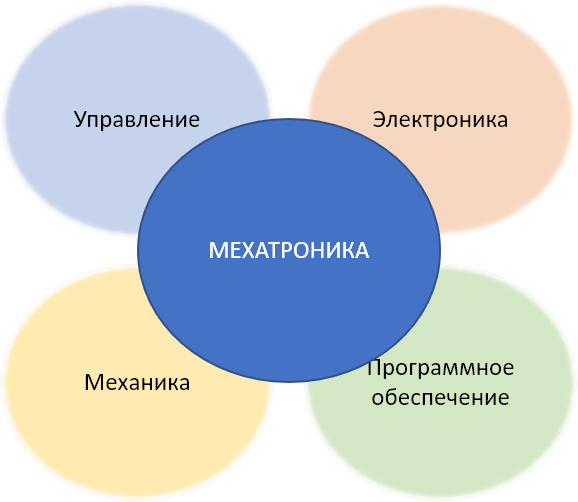
\includegraphics[width=0.5\textwidth]{graphics/Мехатроника.png}

    В рамках курса мы рассматриваем такие аспекты мехатроники, как управление, электроника и программное обеспечение.

    АСУ ТП (автоматизированная система управления технологическим процессом)
    становятся всё менее распространёнными по причинам плохой
    расширяемости (одна система управления на множество датчиков и механизмов).
    На замену АСУ ТП приходят КФС, как более гибкие и надёжные.

    \section{История робототехники}
    \begin{itemize}
        \item Движущиеся статуи (I век до нашей эры)
        \item Механические устройства (Леонардо да Винчи)
        \item Автоматоны (Пьер Жаке-Дро)
        \item Разностная машина (Чарльз Бэббидж)
        \item Boilerplate (Арчи Кемпион)
    \end{itemize}

    \section{Промышленные роботы}
    \begin{itemize}
        \item Манипуляторы
        \item Johns Hopkins Beast (JHB) (1960) — робот, решающий главную задачу всех
              роботов (найти поесть) Он умел искать розетки, от которых
              подзаряжался, в белой комнате с чёрными розетками посредством
              фотоэлемента. При этом робот был полностью кибернетическим и вся
              логика его управления была реализована посредством множества
              транзисторов.
              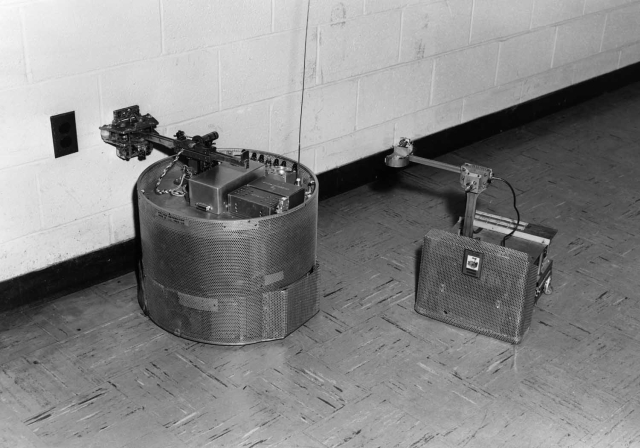
\includegraphics[width=0.7\textwidth]{graphics/johns_beast.jpg}
        \item Shakey (1970) — первый робот, который был способен "думать" над своими действиями.
              Имел на своём борту компьютер и, в отличие от JHB, был способен
              разбивать команды оператора на подзадачи. Например, при
              получении команды «столкни блок с платформы», он осматривал
              окружающее пространство, искал платформу с блоком и пандус, толкал
              пандус к платформе, забирался по нему на платформу и сталкивал
              блок.
        \item Луноход
        \item Марсоход
    \end{itemize}

    Задача грузчика — как двум роботам перенести пианино. Не решённая задача.
    Для решения требуется найти алгоритм нахождения баланса между двумя роботами
    и пианино.

    Робо-рука для сбора помидоров — требует контроля силы сжатия/удержания
    помидора. Несмотря на кажущуюся простоту задачи, тоже до сих пор не
    реализована как раз таки из-за проблем с контролем силы.

    \section{Тенденции развития}
    \begin{itemize}
        \item Разработка стандартов
        \item Уменьшение размеров
        \item Удешевление стоимости комплектующих
        \item Развитие систем управления:
              \begin{itemize}
                  \item ИИ
                  \item Стайное управление
                  \item Функционирование в условиях неопределённости
              \end{itemize}
    \end{itemize}
    \subsection*{Три уровня планирования:}
    \begin{itemize}
        \item Оперативный — решение текущей задачи
        \item Тактический — решение множества задач, для перехода к новому классу задач
        \item Стратегический — главная цель, на которую направлены задачи всех
              остальных уровней
    \end{itemize}

    Пример разделения цели «Получать много денег»:
    \begin{itemize}
        \item Оперативный — Копипаст со Stack Overflow — решение текущей задачи
        \item Тактический — Junior $\rightarrow$ Middle $\rightarrow$ Senior
        \item Стратегический — например, увеличение прибыли
    \end{itemize}

    Разработка стандартов — Разработка правил, по которым можно было бы создать
    ИИ, который гарантированно будет выполнять поставленную ему задачу.

    \section{Система}

    \setstretch{1}
    \[
        \begin{array}{ccccc}
            E              & = & E^{\textit{inf}}               & \cup & E^{phy}                    \\
            \uparrow       &   & \uparrow                       &      & \uparrow                   \\
            \text{система} &   & \text{информационные элементы} &      & \text{физические элементы}
        \end{array}
    \]
    \setstretch{1.8}

    Примеры возможных связей между информационными и физическими элементами:
    \begin{center}
        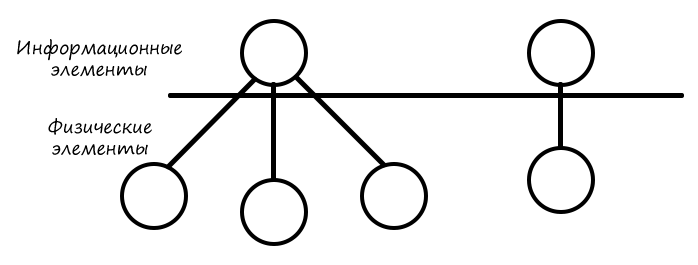
\includegraphics[width=0.5\textwidth]{graphics/Информационные_и_физические_элементы.png}
    \end{center}

    \setstretch{1}
    \[
        \begin{array}{ccccc}
            S_E                      & = & f( & E,             & U)                         \\
            \uparrow                 &   &    & \uparrow       & \uparrow                   \\
            \text{состояние системы} &   &    & \text{система} & \text{входные воздействия}
        \end{array}
    \]
    \setstretch{1.8}

    \setstretch{1}
    \[
        \begin{array}{ccccc}
            U                          & = & U_{\textit{out}} & \cup & U_{in}            \\
            \uparrow                   &   & \uparrow         &      & \uparrow          \\
            \text{Входные воздействия} &   & \text{внешние}   &      & \text{внутренние}
        \end{array}
    \]
    \setstretch{1.8}

    \begin{center}
        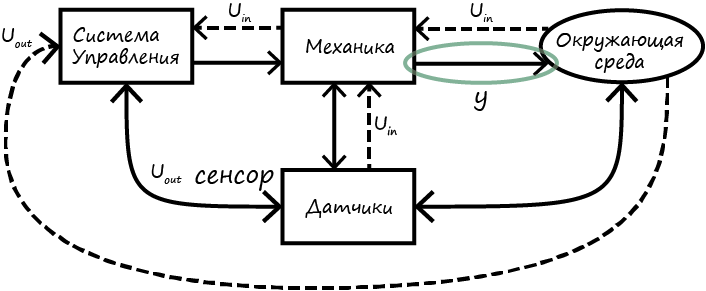
\includegraphics[width=0.7\textwidth]{graphics/Система.png} \\
        Общее устройство системы
    \end{center}


    \begin{center}
        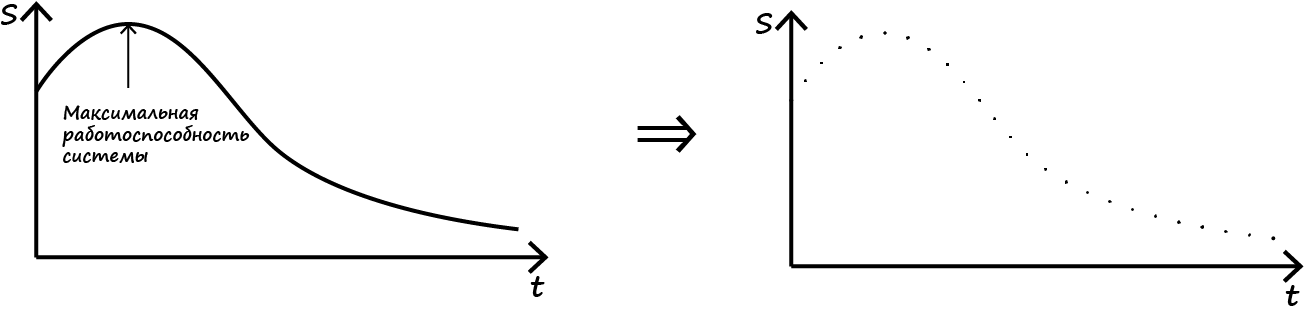
\includegraphics[width=0.9\textwidth]{graphics/Состояние системы.png}
        Дифференцирование состояния системы
    \end{center}

    $y$ — выходные параметры

    $|y| = |U|$. Или, другими словами, размерность $y$ = размерность $U$

    $\dfrac{\delta S}{\delta t} = F(E^t, U^t)$ - состояние системы в конкретный
    момент времени есть функция от системы и входных воздействий в этот же
    момент времени.

    $S_E = y + e$, где $e$ - погрешность системы и обычно опускается, т. к.
    зависит от физических параметров, таких, как качество канала связи.

    При стремлении длины временного отрезка к 0, изменение системы тоже стремится к 0:
    \[
        \Delta r \rightarrow 0 \Leftrightarrow \Delta S \rightarrow 0
    \]

    Когда состояние системы близко к оптимальному, значения выходных параметров стремятся к нормальному распределению.

    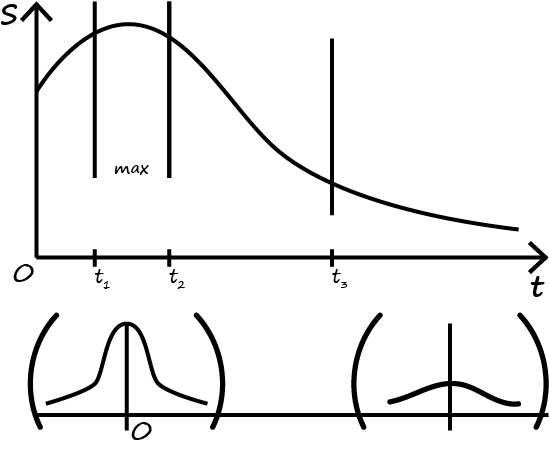
\includegraphics[width=0.5\textwidth]{graphics/Состояния системы и нормальное распределение.png}

    \[
        f: S_E^{\text{норм}} \rightarrow S_E^{\text{плохо}} \text{ — система
            постепенно деградирует, её состояние ухудшается}
    \]

    \section{Виды архитектур интеллектуальных агентов:}
    \subsection{Реактивные}
    Пример - Johns Hopkins Beast.

    \begin{picture}(200,200)
        \thicklines
        \put(100,10){\line(0,1){180}}
        \put(10,100){\line(1,0){180}}
        \put(100,190){\makebox(0,0)[b]{\textsc{Сенсоры}}}
        \put(190,100){\makebox(0,0)[l]{\rotatebox{-90}{\textsc{Реакция}}}}
        \put(100,10){\makebox(0,0)[t]{\textsc{Механика}}}
        \put(10,100){\makebox(0,0)[r]{\rotatebox{90}{\textsc{Словарь действий}}}}
    \end{picture}

    \subsection{Делиберативные}
    Пример - Яндекс Навигатор

    \begin{picture}(200,200)
        \thicklines
        \put(100,10){\line(0,1){180}}
        \put(10,100){\line(1,0){180}}
        \put(100,190){\makebox(0,0)[b]{\textsc{Сенсоры}}}
        \put(190,100){\makebox(0,0)[l]{\rotatebox{-90}{\textsc{Критерий}}}}
        \put(100,10){\makebox(0,0)[t]{\textsc{Механика}}}
        \put(10,100){\makebox(0,0)[r]{\rotatebox{90}{\textsc{Априорная информация}}}}
    \end{picture}

    \subsection{Гибридные}

    Пример - автопилот Tesla (он знает, что нужно делать (априорная информация) (ехать, соблюдая ПДД) и реагирует на изменения (пешеход выбежал на дорогу))

    \section{Сопутствующие задачи для беспилотника:}
    \subsection{Стабилизация}
    Система должна стремиться находится максимально близко к идеальному состоянию.

    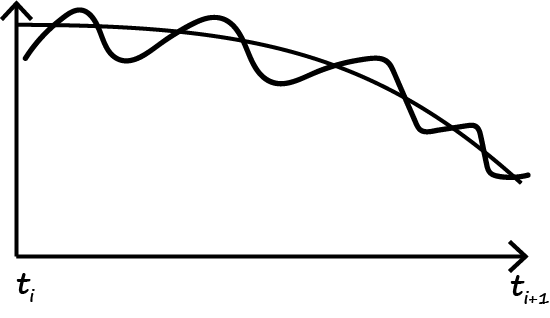
\includegraphics[width=0.5\textwidth]{graphics/Стабилизация.png}

    $y(t) \rightarrow y_* \text{ или } \lim_{t \rightarrow \infty}{|y_* - y(t)|}
        \leq \nu$, где $\nu$
    - допустимое отклонение, а $y_*$ - идеальное состояние.
    Также иногда рассматривается цель вида $\lim_{t \rightarrow \infty}{M|y_* -
            y(t)|} \leq \nu$, где $M$ - символ взятия математического ожидания.
    Второй способ используется когда на объект воздействуют случайные возмущения
    или помехи.  Математическое ожидание позволяет сгладить подобные помехи.

    Классическим примером устройства, решающего подобную задачу является ПИД
    регулятор.

    \subsection{Слежение}
    Система должна сохранять хоть какую-то работоспособность.
    Например - при потере управляющего сигнала дроном.

    $\lim_{t \rightarrow \infty} |U_*(t) - U(t)| = 0$ — функция состояния
    объекта управления (входного состояния системы ($U(t)$)) не должна
    отклонятся от желаемой функции входного состояния системы ($U_*(t)$).
    Другими словами, состояние объекта управление в момент времени $t$ должно
    соответсвовать желаемому состоянию объекта в этот момент времени. Это
    желаемое состояние обычно описывается эталонной моделью.

    \subsection{Возбуждение (разгон, раскачка) колебаний}
    Предполагается, что система изначально находится в состояние покоя и
    необходимо привести её в колебательное движение с заданными
    характеристиками.

    Формально, данную задачу можно свести к задаче слежения.

    $\lim_{t \rightarrow \infty} |G(U(t))| = G_*$, где $G(x)$ - некоторая
    \textbf{скалярная} целевая функция, а $G_*$ - её идеальное значение при
    достижении цели управления.

    \subsection{Синхронизация}
    Система должна быть наблюдаема и повторяема. То есть если создать вторую
    такую же систему, то её можно будет привести в такое состояние, что
    $\forall t \geq 0,\ y_1(t) = y_2(t)$, где $y_1$ и $y_2$ — состояния
    соответствующих систем.

    \section{Рекомендуемая литература}
    \begin{itemize}
        \item Martsenyuk V. P. et al. Software Complex in the Study of the Mathematical Model of Cyber-Physical Systems //ICTES. – 2020. – С. 87-97.
        \item Legatiuk D. et al. A categorical approach towards metamodeling cyber-physical systems //The 11th International Workshop on Structural Health Monitoring (IWSHM). Stanford, CA, USA. – 2017. – Т. 12. – С. 2017.
        \item Platzer A. Logic \& proofs for cyber-physical systems //Automated Reasoning: 8th International Joint Conference, IJCAR 2016, Coimbra, Portugal, June 27–July 2, 2016, Proceedings 8. – Springer International Publishing, 2016. – С. 15-21.
        \item Letichevsky A. A. et al. Cyber-physical systems //Cybernetics and Systems Analysis. – 2017. – Т. 53. – С. 821-834.
        \item Wan J. et al. From machine-to-machine communications towards cyber-physical systems //Computer Science and Information Systems. – 2013. – Т. 10. – №. 3. – С. 1105-1128.
        \item Фрадков А. Л. Кибернетическая физика: принципы и примеры. – 2003.
    \end{itemize}


\end{sloppypar}
\end{document}